\section{Valutazione delle performance dei modelli supervisionati}

L’errore calcolato sul training set non è un buon indicatore delle performance su dati futuri (in quanto i nuovi dati probabilmente non saranno gli stessi dei dati di training).
\begin{itemize}
    \item \textit{Overfitting}: il modello si adatta troppo precisamente ai dati di training generando risultati scarsi su nuovi dati. Si ha un’alta complessità computazionale.
    \item \textit{Underfitting}: il modello si adatta poco ai (è inadatto per i) dati di training generando risultati scarsi su nuovi dati. Si ha una ridotta complessità computazionale.
\end{itemize}

\begin{figure}[H]
    \centering
    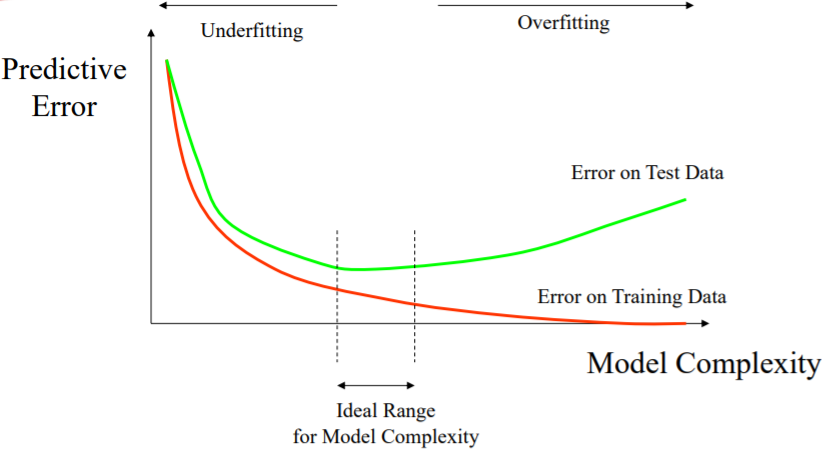
\includegraphics[scale=0.7]{imm/model_complexity.png}
\end{figure}

In mezzo si ha un buon compromesso tra accuratezza (e quindi tasso di errore) e complessità del modello.\\

Le tradizionali misure di performance per i problemi di classificazione sono le seguenti:
\begin{itemize}
    \item \textbf{success (successo)}: la classe di un’istanza è predetta correttamente.
    \item \textbf{error (errore)}: la classe di un’istanza non è predetta correttamente.
    \item \textbf{Error rate (tasso d’errore)}: proporzione di errori compiuti sull’intero set di istanze.
    \item \textbf{Accuracy (accuratezza)}: proporzione di istanze correttamente classificate su tutto il set dell’istanze.
\end{itemize}
Certamente ci sono altre modalità per calcolare la performance, ma questi sono quelli più gettonati/frequenti. 
% 
\begin{table}[H]
\centering
    \begin{tabular}{ll|l|l|}
        \cline{3-4}
        \multicolumn{2}{l}{\multirow{2}{*}{}} & \multicolumn{2}{|c|}{Predicted Class}               \\ \cline{3-4} 
        \multicolumn{2}{l}{}                  & \multicolumn{1}{|c }{Yes} & \multicolumn{1}{c|}{No} \\ \hline
        \multicolumn{1}{|l|}{\multirow{2}{*}{\begin{tabular}[c]{@{}l@{}}Actual  \\ class\end{tabular}}} & Yes & TP:true positive & Fn: False negative \\ \cline{2-4} 
        \multicolumn{1}{|l|}{}      & No      & FP: false positive       & TN: True negative       \\ \hline
    \end{tabular}
\end{table}

I metodi di machine learning solitamente tendono a minimizzare FP+FN. Nella pratica FP e FN possono avere costi diversi.\\

In un problema multiclasse, la matrice di confusione diventa:

\begin{table}[H]
\centering
\begin{tabular}{l|l|l|l|}
\cline{2-4}
 &
  $Class_1$ &
  $\cdots$ &
  $Class_n$ \\ \hline
\multicolumn{1}{|l|}{$Class_1$} &
  \begin{tabular}[c]{@{}l@{}}numero di elementi della classe 1 \\ predetti come elementi della classe 1\end{tabular}&
  $\cdots$ &
  \begin{tabular}[c]{@{}l@{}}numero di elementi della classe 1 \\ predetti come elementi della classe n\end{tabular} \\ \hline
\multicolumn{1}{|c|}{$\vdots$} &
   \multicolumn{1}{c|}{\vdots} &
  $\ddots$ &
  \multicolumn{1}{c|}{\vdots} \\ \hline
\multicolumn{1}{|l|}{$Class_n$} &
  \begin{tabular}[c]{@{}l@{}}numero di elementi della classe n \\ predetti come elementi della classe 1\end{tabular} &
  $\cdots$ &
  \begin{tabular}[c]{@{}l@{}}numero di elementi della classe n \\ predetti come elementi della classe n\end{tabular} \\ \hline
\end{tabular}
\end{table}

Gli elementi della diagonale sono i veri positivi, la riga di una classe è formata dai suoi falsi negativi e la colonna dai falsi positivi.

\subsection{Misure di performance tradizionali (globali)}

\begin{itemize}
    \item \textbf{Accuracy}: $\displaystyle \frac{TP+TN}{TP+TN+FP+FN}$
    \item \textbf{Precision}: $\displaystyle \frac{TP}{TP+FP}$	
    \item \textbf{Recall}: $\displaystyle \frac{TP}{TP+FN}$
    \item \textbf{F-measure}: $\displaystyle \frac{2 \cdot \text{Precision} \cdot \text{Recall}}{\text{Precision} + \text{Recall}}$
\end{itemize}

Nel caso di modelli multiclasse Precision, Recall e F-measure vengono calcolati specificatamente per una classe (non dell’intero modello). Solitamente si calcolano quindi Precision, Recall e F-measure per ogni classe e si calcola poi il valore medio.

\subsection{Misure di performance a livello di classe}

Data un’etichetta $l$ appartenente a un set $L$ di label:
\begin{itemize}
    \item \textbf{Precision}: $P(l) = \displaystyle \frac{\text{numero di istanze correttamente predette come  } l}{\text{numero di istanze predette come }l}$
    \item \textbf{Recall}: $R(l) = \displaystyle \frac{\text{numero di istanze correttamente predette come  } l}{\text{numero di istanze della classe }l}$
    \item \textbf{F-measure}: $F(l) = \displaystyle \frac{2 \cdot P(l) \cdot R(l)}{P(l) + R(l)}$
    \item \textbf{Macro-average}: $Perf^* = \displaystyle \frac{1}{|L|} \sum_{l=1}^{|L|} \cdot Perf(l)$, in questo caso tutte le classi sono equamente importanti
    \item \textbf{Micro-average}: $Perf^* = \displaystyle \sum_{l=1}^{|L|} \frac{|class(l)|}{\text{numero totale delle istanze}} \cdot Perf(l)$. \\ In questa situazione invece le classi predominanti (più corpose) sono le più importanti (media pesata)
\end{itemize}

Oltre ai metodi tradizionali si possono utilizzare le ROC curve. Le \textit{ROC (Receiver Operating Characteristic) curve} sono, in parole povere, delle curve che vengono plottate graficamente mostrano le performance di un classificatore ovvero la sua capacità discriminativa al variare di una determinata soglia.\\

Venie paragonato il rate dei veri positivi al rate dei falsi positivi al variare di una certa soglia.
\begin{figure}[H]
    \centering
    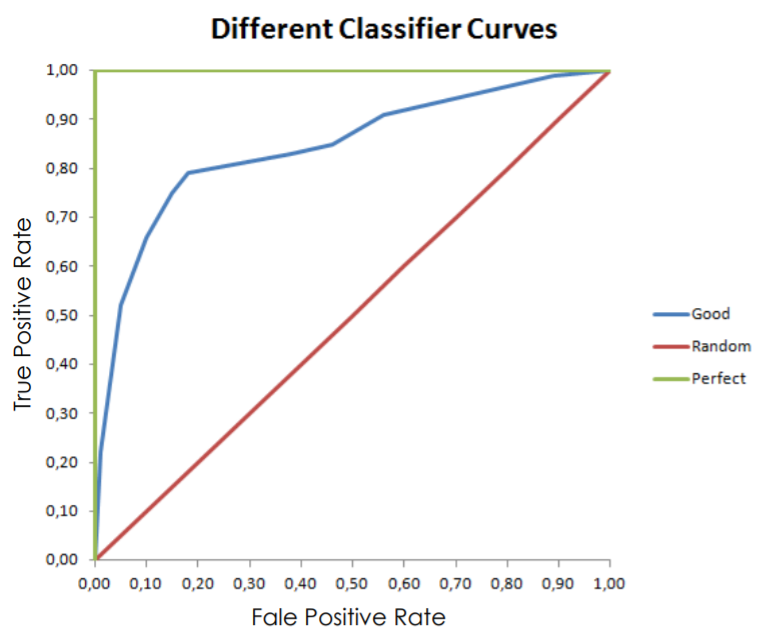
\includegraphics[scale=0.7]{imm/ROC_curve.png}
    \label{fig:roc_curve}
\end{figure}

Di curve ROC, ce ne è una per classe.

Ci sono inoltre le curve di apprendimento (\textit{learning curve}), queste curve ci mostrano invece come l’accuratezza (o un’altra misura di performance) cambia al variare della dimensione del campione. Sono uno strumento per evitare di andare in overfitting.\\

\begin{figure}[H]
    \centering
    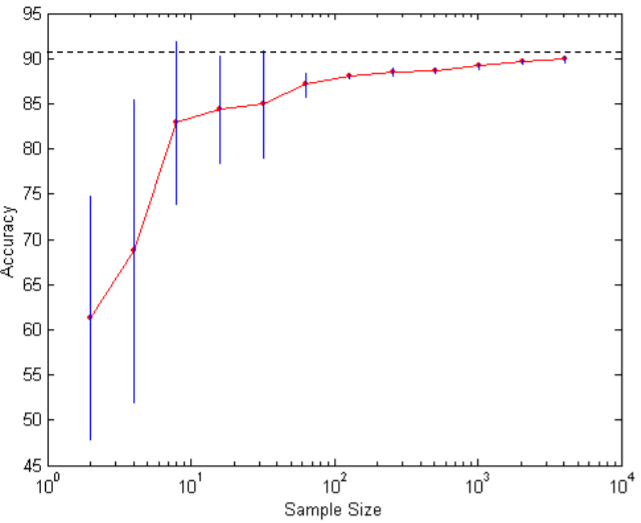
\includegraphics[scale=0.7]{imm/learning_curve.png}
    \label{fig:learning_curve}
\end{figure}
La linea rossa indica il variare dell’accuratezza al variare della dimensione dell’input. Le linee blu mostrano la varianza della performance.\\
A un certo punto al crescere dei dati non aumenta più la performance. \\

Se sono disponibili molti dati, e quindi molti esempi per ogni classe, è possibile convalidare il metodo di classificazione effettuando una semplice suddivisione randomica dei dati in training e test set (solitamente i dati sono divisi in $\frac{2}{3}$ training e l’$\frac{1}{3}$ test. \\
Si costruisce quindi il classificatore utilizzando il training set e lo si convalida usando il test set.\\

Una volta che si è effettuata la convalida, tutti i dati possono essere utilizzati per costruire il classificatore finale. \\
Generalmente, più dati vengono usati per il training e migliore è il classificatore e più dati vengono usati per il test e più accurata è la stima del tasso di errore. I dati di test non devono essere stati utilizzati per creare il classificatore e nemmeno per il tuning dei parametri.\\

La procedura corretta comprende quindi tre insiemi: i dati di training, i dati per la convalida (il validation set è utilizzato per ottimizzare i parametri) e i dati per il test.

\begin{figure}[H]
    \centering
    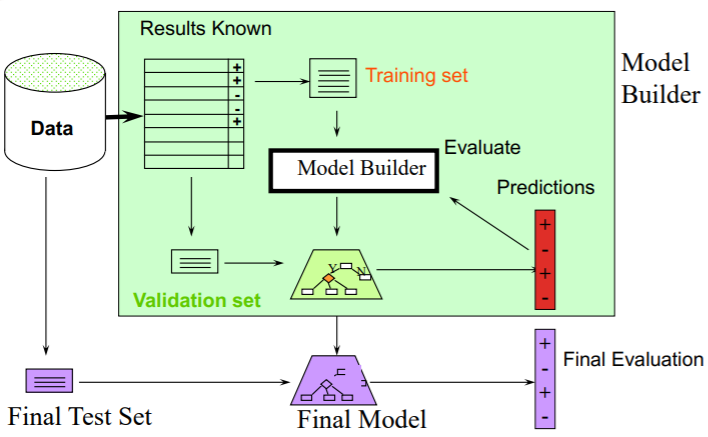
\includegraphics[scale=0.7]{imm/model_builder.png}
    \label{fig:model_builder}
\end{figure}

Nel caso in cui si abbia a che fare con un set di dati ristretto (con il rischio quindi che il training e il test set possano non essere rappresentativi) si utilizza un metodo detto \textit{repeated holdout}.\\

Nel metodo repeated holdout, viene ripetuto il processo di suddivisione in train e test set con diversi sottocampioni: ad ogni iterazione, viene selezionata casualmente una certa proporzione dal training set (possibilmente con stratificazione) e vengono pesate (attraverso una media) le stime d’errore in modo da ottenere una errore stimato globalmente equo.
Il problema è che i diversi test set possono contenere elementi ripetuti. Per risolver questo problema, quello che possiamo fare, è utilizzare una cross-validation.

\subsection{Cross-validation}
Metodo di repeated holdout che evita la sovrapposizione dei test set.
\begin{enumerate}
    \item I dati vengono suddivisi in $k$ sottoinsiemi di egual misura.
    \item Ogni sottoinsieme viene utilizzato a turno per testare e il resto viene usato per il training.
\end{enumerate}
Questo metodo viene chiamato \textit{k-fold cross-validation}. Spesso i sottoinsiemi vengono stratificati prima della cross-validation.

\begin{figure}[H]
    \centering
    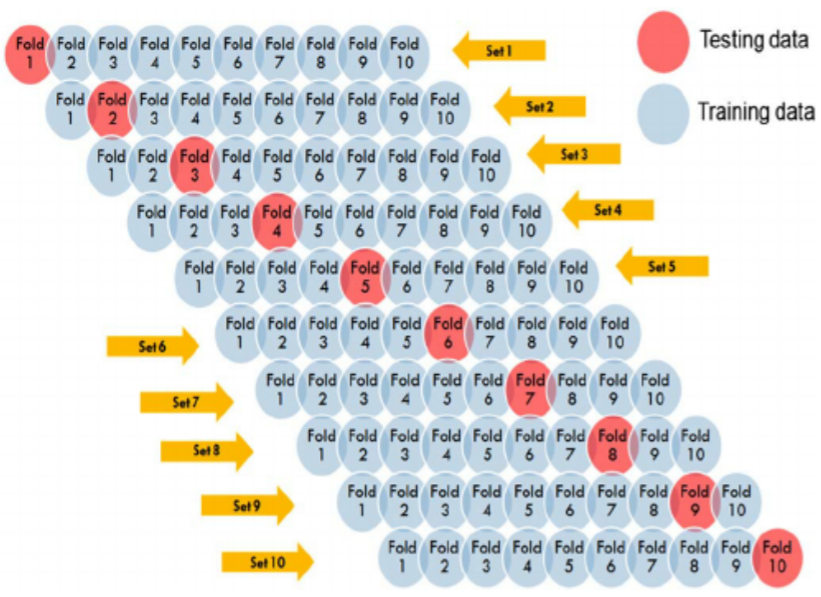
\includegraphics[scale=0.4]{imm/cross_validation.png}
    \label{fig:cross_validation}
\end{figure}

Nel caso in cui si voglia ottenere una matrice di confusione per l’intero 10-fold, si deve calcolare la matrice di confusione per ogni iterazione e poi sommarle.\\
Un metodo standard per la convalida che possiamo andare ad utilizzare è il \textbf{stratified \textit{ten}-fold cross-validation}.  
Con \textit{stratified}, intendiamo dire che la distribuzione delle istanze selezionate in relazione alla classe che dev’essere predetta in ogni fold, è simile alla distribuzione originale del dataset. La stratificazione riduce la varianza delle stime.\\

Una domanda lecita sarebbe chiedersi come mai \textbf{\textit{ten}-fold}. Di norma si usano 10 fold perché è stato dimostrata essere la miglior scelta per ottenere una stima accurata. Un metodo ancora migliore è il repeated stratified cross-validation nel quale la cross-validation è ripetuta $k$ volte e viene considerata la media dei risultati, al fine di ridurre al varianza.\\

\subsection{Bootstrap}
Ci sono altre tecniche, oltre alla cross validation, infatti come abbiamo detto la \textit{cross-validation} effettua il campionamento senza rimpiazzamento. Una stessa istanza, una volta selezionata, non può essere selezionata nuovamente per un determinato training/test set.\\
Mentre ci sono altre tecniche, come Bootstrap. In questa tecnica usa il campionamento con rimpiazzo per formare il training set. Suddivide un dataset di $n$ istanze $n$ volte con rimpiazzamento per formare un nuovo dataset di $n$ istanze che viene utilizzato come training set.Le istanze del dataset originale che non occorrono nel nuovo training set vengono utilizzate per il testing.\\

\subsubsection{0.632 Bootstrap}
Una particolare istanza ha una probabilità di $1 - \displaystyle \frac{1}{n}$ di non essere scelta.
Quindi la probabilità di finire nel test set è del: \[\left( 1- \displaystyle \frac{1}{n} \right)^n \approx e^{-1} = 0.368\]
Ciò significa che i dati di training conteranno approssimativamente il $63.2\%$ delle istanze.\\

Bootstrap tende a ridurre drasticamente la varianza, ma fornisce risultati con bias (tendono ad essere pessimistici).
È adatto a stimare la performance per dataset molto ridotti.

\subsubsection{Leave-One-Out Cross-Validation}
Una particolare forma di cross-validation che setta il numero di fold al numero delle istanze di training (con $n$ istanze di training, costruisce il classificatore $n$ volte). \\
Utilizza meglio i dati, senza coinvolgere sotto campionamenti casuali ma è molto costosa computazionalmente.\\

%%%%%%%%%%% Si aggiunge, dal laboratorio 10

Per sapere quanto si avvicina la stima del tasso di errore al tasso di errore effettivo, è possibile utilizzare gli intervalli di confidenza per capire meglio la proporzione che si sta considerando.\\

\textbf{\textit{Intervallo di confidenza (confidence interval)}}\\
Possiamo dire che $p$ appartiene a uno specifico intervallo con una specifica confidenza. A parità di tasso di errore stimato si sceglie il modello che garantisce un intervallo di confidenza più stretto (ovvero una minor variabilità del risultato).\\

\textbf{\textit{Significance test}}\\
I \textit{significance test} dicono quanto si può essere confidenti del fatto che ci sia effettivamente una differenza tra i risultati di due modelli. Abbiamo due modi per dirlo:
\begin{itemize}
    \item \textbf{Null hypothesis}hypothesis: non c’è una reale differenza.
    \item \textbf{Alternative hypothesis}: c’è una differenza.
\end{itemize}
Un test di significatività misura quanta evidenza c’è nel favorire il rigetto dell’ipotesi nulla.

\subsection{T di Student test}
Questo test ci dice se le medie di due campioni sono significativamente diverse. Consiste nel prendere campioni individuali dal set di tutte le possibili stime di cross-validation.

Si utilizza un t-test \textit{paired}: solo se i campioni individuali sono accoppiati (quindi se viene applicato a entrambi i modelli lo stesso cross-validation). È possibile applicarlo se i due modelli che si stanno testando stanno lavorando esattamente sulla stessa configurazione di fold (stesse istanze, stesse istanze nei fold e le istanze vengono processate esattamente nello stesso modo).\\

C’è una corrispondenza tra le predizioni dei due modelli.

\subsubsection{Calcolo del paired t-test}
Si considerano i campioni (gli elementi da confrontare, solitamente le predizioni) provenienti da un k-fold CV. Vengono normalizzati i dati per poter assumere di avere una distribuzione normale (media 0 e varianza 1). Con un campione dati abbastanza ampio possiamo sicuramente dire che la media di un seti di dati indipendenti è normalmente distribuito. Siano poi le stime di varianza delle medie date da $\frac{\sigma_x^2}{k}$ e $\frac{\sigma_y^2}{k}$, se $\mu_x$ e $\mu_y$ rappresentano le medie dei due campioni, allora: 
\[\displaystyle \frac{m_i - \mu_i} {\sqrt{\displaystyle \frac{\sigma_i^2}{k}}} \quad \mbox{ con } i \in \{x,y\}\],
Le media sono approssimamene normalmente distribuite con media uguale a 0 e varianza pari a 1.\\

Si calcolano $m_d = \mu_x - \mu_y$ (e si assume che anche questa sia distribuita normalmente) e $\sigma_d^2$ come la varianza della differenza. \\
A questo punto si calcola la statistica \[t = \displaystyle \frac{m_d}{\sqrt{\displaystyle \frac{\sigma_d^2}{k}}}\]
Dove $k$ è il numero di fold della $k$-fold cv(cross validation) (si assume che $m_d$ abbia una distribuzione di student con $k-1$ gradi di libertà), e la si usa per eseguire un t-test. Allora in ordine per eseguire il test eseguiamo i seguenti passi:
\begin{enumerate}
    \item Si fissa un livello di significatività $\alpha$ e se una differenza è significativa all’$\alpha\%$ allora c’è una possibilità del $(100-\alpha)\%$ che ci sia davvero una differenza.
    \item Si divide il livello di significatività per 2 perché il test è \textit{two-tailed}, e andiamoa a ritrovare il $z$ value associato al valore calcolato dalla $\alpha/2$.
    \item Se $t \leq -z$ o $t \geq z$ allora la differenza è significativa e quindi l’ipotesi nulla può essere rigettata.
\end{enumerate}

\subsection{Valutazione delle performance dei modelli non supervisionati}

Nella valutazione di una soluzione di clustering è bene considerare due fattori:
\begin{enumerate}
    \item \textit{Clustering tendency}: Bisogna verificare (prima del clustering) che i dati abbiano una tendenza (la clustering tendency) e che non contengano punti uniformemente distribuiti. Esistono due metodi per valutare la clustering tendency: 
        \begin{itemize}
            \item \textit{Hopkins statistic}: valuta la clustering tendency misurando la probabilità che un certo dataset sia generato da una distribuzione di dati uniforme, ovvero testa la spatial randomness dei dati. Sia $D$ un dataset real. La Hopkins statistic può essere calcolata come segue:
                \begin{enumerate}
                    \item Si campionano uniformemente $n$ punti ($p_1, \dots, p_n$) di $D$
                    \item  Si calcola la distanza $x_i$ da ogni punto reale al suo più vicino neighbor. 
                        Per ogni punto $p_i \in D$ si trova il più vicino punto $p_j$ e si computa la distanza tra i due $x_i = dist(p_i, p_j)$.
                    \item  Si genera un dataset simulato $randomD$ creato da una distribuzione uniforme e casuale di $n$ punti $q_1, \dots, q_n$ che abbia la stessa variazione del dataset originale $D$.
                    \item Si computa la distanza $y_i$ da ogni punto artificiale al più vicino punto reale.
                        Per ogni punto $q_i \in randomD$ si trova il più vicino punto $q_j \in D$ e si computa la distanza tra i due $y_i = dist(q_i, q_j)$.
                    \item Si calcola la Hopkins statistic $H$ come il rapporto tra la media delle distanze tra i punti più vicini in $randomD$ e la somma delle distanze medie tra i punti più vicini nel dataset reale e quello simulato.
                \end{enumerate}
                    \[\displaystyle H =  \displaystyle \frac{\displaystyle\sum_{i=1}^n{y_i}}{\displaystyle\sum_{i=1}^n{x_i} + \displaystyle\sum_{i=1}^n{y_i}} \]
            Un valore di $H$ maggiore di $0.75$ indica una clustering tendency con livello di confidenza al $90\%$.
            \item \textit{ Visual Assessment of cluster Tendency} (VAT) algorithm
                \begin{enumerate}
                    \item Si calcola la matrice di dissimilarità (dissimilarity matrix, DM) tra gli oggetti nel dataset usando la misura di distanza euclidea.
                    \item Si riordina la DM in modo tale che oggetti simili siano vicini tra di loro.
                       Questo processo crea una ordered dissimilarity matrix (ODM).
                    \item L’ODM è visualizzata come una ordered dissimilarity image (ODI) che l’output visuale del VAT.
                       \begin{figure}[H]
                            \centering
                            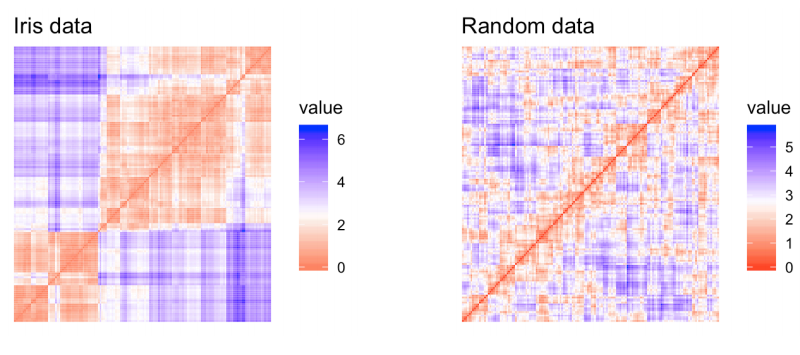
\includegraphics[scale=0.6]{imm/ODM.png}
                            \label{fig:odm}
                        \end{figure}
                \end{enumerate}
        \end{itemize}
    \item \textit{Clustering quality}: possibile utilizzare misure interne (within sum of square, silhouette) e misure esterne, se si hanno anche etichette associate alle istanze, (precision, recall, f-measure). \\
        Nel caso di misure esterne vige il criterio di maggioranza: si associa ad ogni cluster la classe a cui appartiene la maggioranza delle istanze del cluster.
\end{enumerate}